\documentclass[12pt, A4]{article}

% Packages
	% Basics
		\usepackage{amsmath}
		\usepackage{bm}
		\usepackage{cellspace}
		\usepackage{csquotes}
		\usepackage{fixltx2e}
		\usepackage[hang,flushmargin]{footmisc}
		\usepackage{float}
		\usepackage[margin=0.75in]{geometry}
		\usepackage{graphicx}
		\usepackage{hyperref}
		\usepackage[utf8]{inputenc}
		\usepackage{subcaption}
	% Diagrams
		\usepackage{pgfplots}
		\usepackage{tikz}
			\usepackage{circuitikz} % Circuits
			\usepackage{tikz-3dplot} % 3D
			\usetikzlibrary{arrows.meta, angles, calc, quotes}
	% Notation
		\usepackage{amssymb} % Miscellaneous
		\usepackage{chemformula}
		\usepackage{esint} % Integrals
		\usepackage{physics} % Differentials/Vectors
% Configuration
	\title{Differential Equations Project: Phase 3}
	\author{Arnav Patri and Shashank Chidige}
	\hypersetup{
	    colorlinks,
	    citecolor=cyan,
	    filecolor=cyan,
	    linkcolor=cyan,
	    urlcolor=cyan
	}
	\cellspacetoplimit10pt
	\cellspacebottomlimit10pt
	
% Macros
	% Notation
		% Constants
			\DeclareMathOperator{\en}{e}
		% Distributions
			\newcommand{\Exp}{\mathbb{E}}
			\newcommand{\ndist}{\mathcal{N}}
			\DeclareMathOperator{\vari}{var}
		% Functions
			\DeclareMathOperator{\erfc}{erfc}
		% Sets
			\newcommand{\R}{\mathbb{R}}
		% Other
			\DeclareMathOperator{\avg}{avg}
			\renewcommand{\th}{\text{th}}
	% Utilities
		\newcommand{\callout}[2]{\begin{center}\fbox{\begin{minipage}{#1cm}#2\end{minipage}}\end{center}}
		\newcommand{\comment}[1]{}
		\newcommand{\subsectionb}[1]{\subsection*{#1}\addcontentsline{toc}{subsection}{#1}}
		\newcommand{\subsubsectionb}[1]{\subsubsection*{#1}\addcontentsline{toc}{subsubsection}{#1}}

\begin{document}
	\maketitle
	\noindent
	This is the dependent variable Stock Price of Alphabet (\(S\)) and the independent variable Days (\(t\)). The data is taken from Yahoo Finance from the ticker GOOG. 
	\[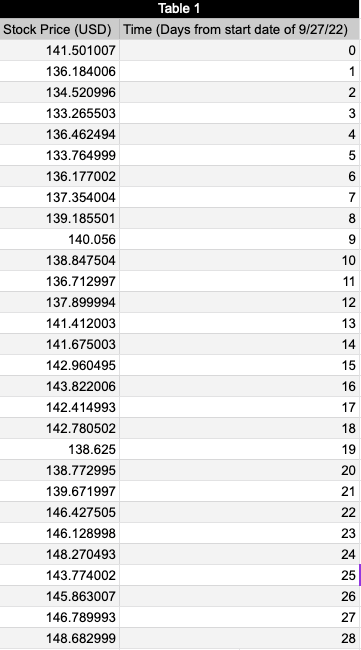
\includegraphics[width = 9cm]{Images/Table_1}\]
	This table calculates the changes in each variable.
	\[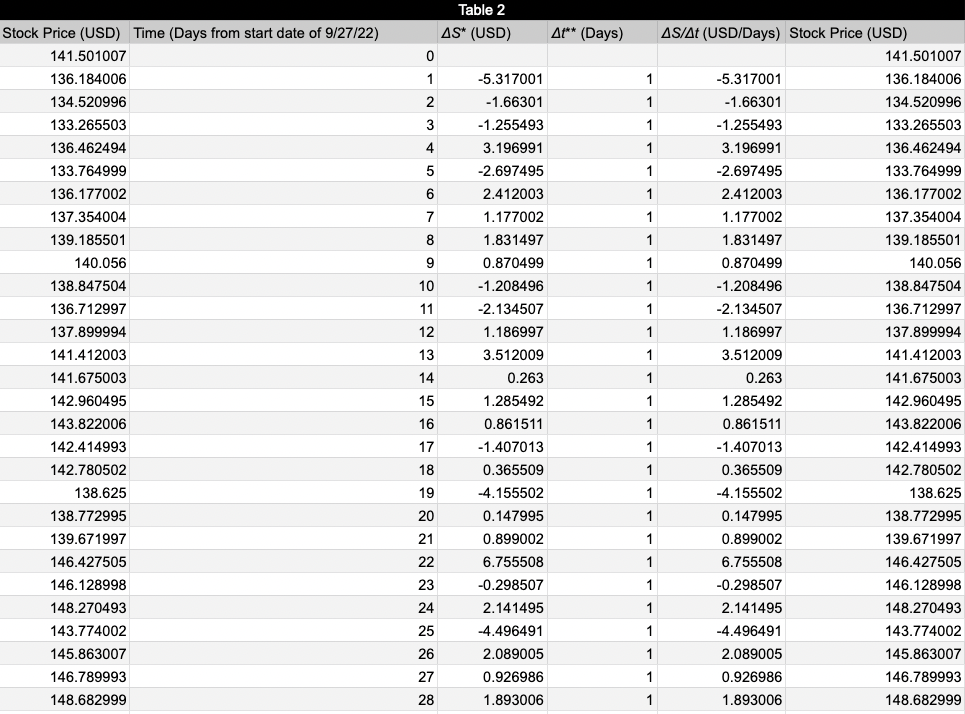
\includegraphics[width = 18cm]{Images/Table_2}\]
	\begin{align*}
		\Delta S_i &= S_i - S_{i - 1} \tag{Equation 1*} \\
		\Delta t_i &= t_{i} - t_{i - 1} \tag{Equation 2**}
	\end{align*}
	This is the graph of \(\Delta S/\Delta t\) (in USD/day) vs \(S\) (in USD) with a linear regression performed.
	\[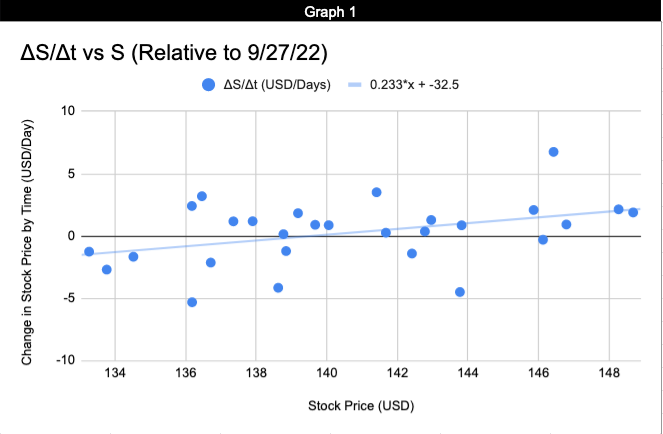
\includegraphics[width = 10cm]{Images/Graph_1}\]
	The DE being used to model stock price is
		\[\dv{S_t}{t} = \mu S_t + \sigma S_t\dv{W_t}{t}\]6
		where \(S_t\) is stock price as a function of time \(t\), \(\mu\) is the (constant) drift, \(\sigma\) is the (constant) volatility, and \(W_t\) is a standard Wiener process. The dependent variable \(t\) is not present, making this an autonomous DE. The only information needed for the model are \(\mu\), \(\sigma\), and the initial stock price \(S_0\). \\
	\(\mu\) is the amount that \(\Exp(S)\) changes per year, making it the coefficient of the linear regression of \(\Delta S/\Delta t\) against \(S\) divided by 365, so \(\mu \approx 0.00064\). \\
	\(\sigma\) is simply the standard deviation of the stock price in the sample, so \(\sigma \approx 4.356\). \\
	The model then becomes
		\[\boxed{\dv{S_t}{t} = 0.00064S_t + 4.356S_t\dv{W_t}{t}}\]
		
\end{document}
